
\section{Introduction}

Recently, an increasing number of organizations are tracking information across
social media and the web.
To this end, the National Institute of Standards hosted a three-year
track to accelerate the extraction of information and construction of knowledge bases from streaming web
resources~\cite{frank2013evaluating}.
This international contest highlighted the many difficulties of dealing with collecting 
unstructured data across the web.
Across these efforts in this contest, we identify entity resolution as a major barrier to progress. 


% Why is the problem hard
Entity resolution across text corpora is the task of identifying mentions 
within the documents that correspond to the same real-world entities.
To construct knowledge bases or extract accurate information, entity resolution (ER) is a required step.
This task is a notoriously computationally difficult problem.
In sampling-based ER, using Markov Chain Monte Carlo (MCMC) techniques exchanges raw performance for a flexible representation 
and guaranteed convergence~\cite{mccallum03towardconditional,singh2011large,wick2013discriminative}.
%Several efforts in different domains have made outstanding progress.

Processing streaming textual documents exacerbates two of the core difficulties of ER.\@
First, the computation of large entities and second, excessive
computation spent resolving unambiguous entities.
Over time, the growing size of large entities makes keeping up with the incoming documents untenable.
Optimization that touches these critical portions is wholly understudied.
In this paper, we argue that compression and approximation 
techniques can efficiently decrease the runtime of traditional ER systems thus
making them usable for streaming environment.

In sampling-based entity resolution, entities are represented as clusters of mentions.
A proposal is made to move a random mention from a source entity to a random destination entity.
The proposed state is scored and if it improves the global state, the new state is accepted.
If the proposal does not improve the global state, the proposal may still be accepted with some small probability.
This process is repeated until the state converges.
Scoring the state of an entity cluster, through pairwise feature computation of the cluster mentions, is $O(n^2)$.
For entity clusters larger than 1000 mentions, calculating the score for each proposal can become prohibitively expensive.
%Performing overly sophisticated techniques over many small clusters could also 
%add extra overhead.

% What are the technical challenges and validation
Wick et al.\ present an entity resolution system that uses a tree structure
to organize related entities to reduce the amount of work performed in each step~\cite{wick2013discriminative}.
During each proposal, this approach avoids the pairwise comparison by restricting model calculation to the top nodes of the hierarchy.
This approach can avoid massive amounts of computation by performing organizing the known sets of mentions.
This discriminative tree structure is a type of \textit{compression}.

Singh et al.\ present a method of efficiently sampling factors to reduce the
amount of work performed when computing features~\cite{singh2012monte}.
They observe that many factors are redundant and do not need to be computed when calculating the feature score.
They use statistical techniques to estimate the computed feature scores with a user-specified confidence.
This approach can be categorized as \textit{early stopping} for feature computation.
% http://people.cs.umass.edu/~sameer/files/mcmcmc-emnlp12-ppt.pdf

There is no one size fits all sampling algorithm~\cite{sculley2006compression};
each of these methods, compression and early stopping, has drawbacks.
Compression may slow down insertion speed and requires extra book keeping to keep to organize the data structure.
Early stopping is not always precise and adding an extra conditions in the metropolis hastings loop structure may slow down computation.
Applying each technique at appropriate times can remove pain points and accelerate the entity resolution process.

% How we differ
In this paper, we discuss our initial work towards the design of an optimizer that modifies the
sampling-based collective entity resolution process to improve sampling performance.
Static parameters for evaluating entity resolution rarely hold for the lifetime of streaming processing task.
The optimizer, in the spirit of the \textit{eddy} database query optimizer~\cite{avnur2000eddies}, dynamically examines the
current state of each proposal and suggests methods for evaluating proposals and structuring entities.
We train a classifier to decide when the sampling process should use early stopping.
Additionally, we use training data to decide when is the best time for a particular entity to be compressed.
This is done with negligible book keeping and a small book keeping over head.
We make the following contributions:
\begin{itemize}
\item We identify several techniques to speed up sampling past a natural baseline.
\item We create rules and techniques for an optimizer to choose parameters and methods at run time.
\item We empirically evaluate these methods over a large data set.
\end{itemize}
We recognize that optimizers can also apply to many different long running machine learning pipeline.
Figure~\ref{fig:optimizer-arch} depicts that the optimizer supervises the machine learning model.
The optimizer determines the methods of processing the streaming updates of the model. 
As future work, we plan to create a full optimizer to study performance improvements on long running machines learning tasks.


\begin{figure}
\centering
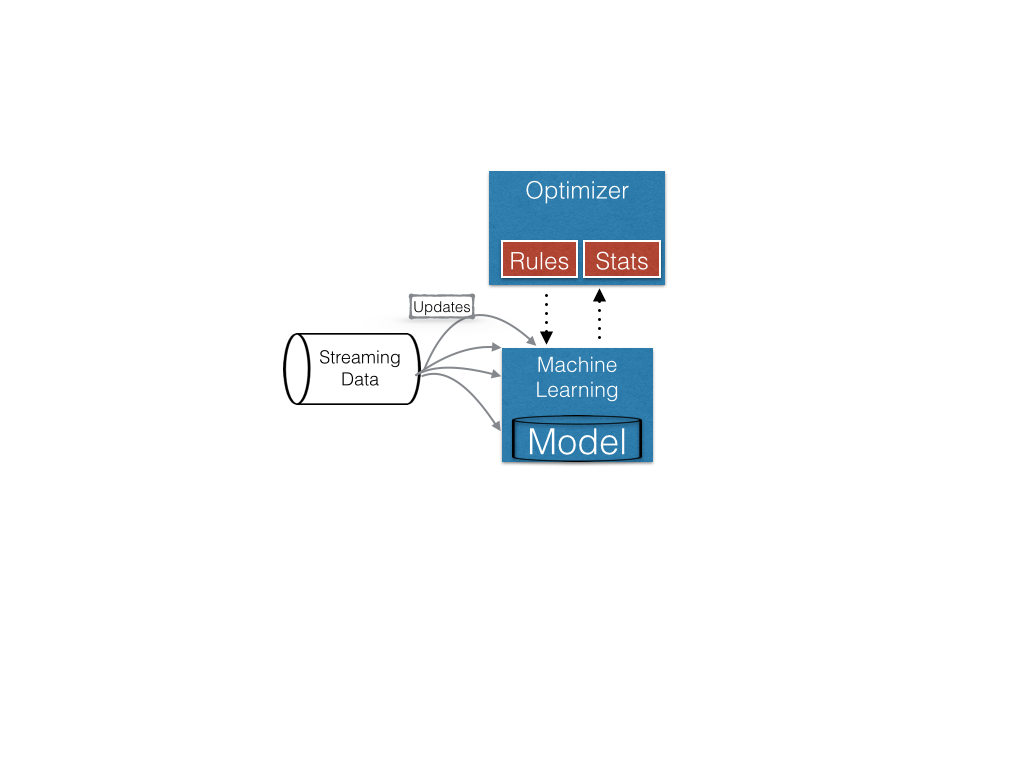
\includegraphics[width=\columnwidth, clip=true, trim= 25em 30em 30em 17em]{media/optimizer/optimizer.png}
\caption{The high-level interaction of the optimizer. As streaming data updates pass to the machine learning model, the optimizer recommends the best algorithms to update the model. Entity resolution is an example of a model that needs to be frequently updated with new data.}
\label{fig:optimizer-arch}
\end{figure}


The outline of the paper is as follows.
In Section~\ref{sec:optimizer:background}, we give a introduction to factor graph models and entity resolution.
In Section~\ref{sec:optimizer:relatedwork}, we discuss three papers that can possibly benefit from an optimizer.
In Section~\ref{sec:optimizer:example}, we further discuss the statistics that an optimizer for entity resolution can use.
In Sections~\ref{sec:optimizer:algorithms} and~\ref{sec:optimizer:optimizer}, we discuss the implementation of the optimizer.
Finally, in Section~\ref{sec:optimizer:implementation}, we examine
the benefits by testing early stopping and compression over a synthetic and a popular real world entity resolution data set.


% Links to people who used vectorization
% http://citusdata.github.io/cstore_fdw/
% http://www.drdobbs.com/parallel/parallel-in-place-merge-sort/240169094?pgno=2

